\documentclass[runningheads]{llncs}
\usepackage[utf8]{inputenc}
\usepackage[T1]{fontenc}
\usepackage[english]{babel}
\usepackage{amsmath,amssymb}
\usepackage{float}
\usepackage{graphicx}
\usepackage{url}
% Keep compilation usable when optional experiment figures are not checked out.
\let\originalincludegraphics\includegraphics
\renewcommand{\includegraphics}[2][]{%
  \IfFileExists{#2}{%
    \originalincludegraphics[#1]{#2}%
  }{%
    \fbox{\small Missing image: \texttt{\detokenize{#2}}}%
  }%
}
\usepackage{booktabs}
\usepackage{array}
\newcommand{\code}[1]{\texttt{#1}}

\begin{document}
\title{The Impact of Convex Free-Space Decomposition on Graphs of Convex Sets for Motion Planning}
\titlerunning{Convex Decompositions for GCS--B\'ezier Planning}
% TODO: Replace the template author and affiliation metadata before submission.
\author{First Author\inst{1}\orcidID{0000-1111-2222-3333} \and
Second Author\inst{2,3}\orcidID{1111-2222-3333-4444} \and
Third Author\inst{3}\orcidID{2222--3333-4444-5555}}
%
\authorrunning{F. Author et al.}
% First names are abbreviated in the running head.
% If there are more than two authors, 'et al.' is used.
%
\institute{Princeton University, Princeton NJ 08544, USA \and
Springer Heidelberg, Tiergartenstr. 17, 69121 Heidelberg, Germany
\email{lncs@springer.com}\\
\url{http://www.springer.com/gp/computer-science/lncs} \and
ABC Institute, Rupert-Karls-University Heidelberg, Heidelberg, Germany\\
\email{\{abc,lncs\}@uni-heidelberg.de}}
%
\maketitle
%
\begin{abstract}
Graphs of Convex Sets (GCS) coupled with B\'ezier trajectories provide a
convex-optimization-based framework for collision-free motion planning, but
their efficiency depends on the convex cover of free space.
We investigate how the cover-construction method affects the downstream GCS
model by comparing Approximate Convex Decomposition (ACD) and Visibility Clique
Cover (VCC) within the same GCS--B\'ezier pipeline. The benchmark
uses five planar map families with five randomized instances per family and
measures decomposition cost, graph and model size, planning time, robustness,
and trajectory quality. ACD solves all 25 instances, whereas VCC solves 23; both
failures occur in narrow passages. On \code{clustered} maps, VCC reduces median
region and edge counts from 104 to 22 and from 462 to 99 and the median GCS solve
time from 40.10~s to 3.10~s. Under the
tested sampling configuration, however, VCC's higher decomposition cost makes
ACD faster end-to-end on every map family. Across 48 successful runs, edge count
correlates more strongly with solve time than region count ($\rho=0.982$ versus
$\rho=0.839$). VCC yields higher median minimum clearance in each successfully
solved family but does not consistently improve path length or traversal time.
These results indicate that edge count is a more informative
predictor of GCS difficulty than region count alone. For the tested single-query
setting, ACD is the more reliable and faster default; VCC may be advantageous
when its construction cost can be amortized or when it substantially reduces
graph connectivity.

\keywords{Motion planning \and Graphs of Convex Sets \and B\'ezier trajectories
\and convex free-space decomposition \and visibility clique cover}
\end{abstract}
%

%
%
\section{Introduction}
Motion planning requires a robot to reach a goal while remaining collision-free
and respecting its motion constraints. This task is challenging because obstacles
make the free configuration space non-convex. Sampling-based planners, such as
probabilistic roadmaps and rapidly exploring random trees, can explore complex
spaces effectively~\cite{KavrakiEtAl1996,LaValle1998}; trajectory-optimization
methods can generate smooth motions but commonly depend on a feasible
initialization and may converge to a local solution
~\cite{Zucker2013_CHOMP,Schulman2014_TrajOpt}. Methods that expose convex
structure in the free space offer a complementary route to handling this
geometric non-convexity.

Graphs of Convex Sets (GCS) formulate motion planning as a joint discrete and
continuous optimization problem~\cite{MarcucciEtAl2023GCS}. A collision-free
free-space cover is represented by convex regions and their feasible
transitions; GCS then selects a route through this graph while optimizing the
trajectory within the chosen regions. When combined with B\'ezier curves, the
convex-hull property provides continuous-time collision guarantees from convex
containment constraints~\cite{MarcucciEtAl2023MotionPlanning}. The quality of
the convex cover is therefore central to practical performance. It controls not
only the number of regions, but also their overlap pattern, the number of GCS
edges, and ultimately the size of the optimization problem.

This paper studies that front-end design choice by comparing Approximate Convex
Decomposition (ACD)~\cite{LienAmato2006} and Visibility Clique Cover
(VCC)~\cite{DeitsTedrake2023VCC} in the same GCS--B\'ezier planning pipeline.
ACD uses local concavity to decompose polygonal free space, whereas VCC uses
sampled visibility and convex-region inflation to seek a compact cover. These
methods embody different trade-offs: ACD can be inexpensive to construct but may
yield many local regions, while VCC can reduce the downstream graph but incurs
sampling and clique-cover costs and can be sensitive to narrow passages.

We make the following empirical contributions:
\begin{itemize}
  \item We provide a paired comparison of ACD and VCC on five two-dimensional
  map families, using five randomized instances per family and a common
  GCS--B\'ezier planner.
  \item We evaluate decomposition time, GCS graph and presolved-model size,
  solve time, end-to-end time, success rate, and trajectory quality rather than
  using the number of regions as the sole proxy for performance.
  \item We show that, in this benchmark, the induced edge structure is more
  strongly associated with GCS solve time than region count alone. ACD provides
  the more reliable and faster single-query pipeline, whereas VCC may be useful
  when its construction can be amortized across repeated queries or when it
  substantially reduces graph connectivity.
\end{itemize}

The remainder of the paper is organized as follows.
Section~\ref{sec:technical-background} summarizes the GCS free-space
representation and the two decomposition methods.
Section~\ref{sec:gcs-bezier-framework} presents the GCS--B\'ezier planning
framework. Section~\ref{sec:experiments} reports the experimental evaluation,
and Section~\ref{sec:conclusion} concludes the paper and outlines future work.

\section{Technical Background}
\label{sec:technical-background}

\subsection{Convex Free-Space Covers for GCS--B\'ezier}
\label{sec:convex-free-space}

Obstacle avoidance makes motion planning difficult because the free
configuration space $\mathcal{C}_{\mathrm{free}}$ is generally non-convex.
The GCS--B\'ezier approach addresses this difficulty by representing the
part of $\mathcal{C}_{\mathrm{free}}$ relevant to a query with a finite
collection of collision-free convex regions,
\[
  \mathcal{Q}=\{Q_i\}_{i=1}^{N_R}, \qquad
  Q_i \subseteq \mathcal{C}_{\mathrm{free}}.
\]
The regions may overlap. They induce a graph with one vertex per region and an
edge for each feasible transition between adjacent regions. The start and goal
are connected to the regions that contain them or can be reached from them.

Graphs of Convex Sets (GCS) jointly optimize the discrete route through this
graph and the continuous trajectory variables associated with the selected
regions~\cite{MarcucciEtAl2023GCS,MarcucciEtAl2023MotionPlanning}. In the
GCS--B\'ezier formulation, a trajectory segment is represented by B\'ezier
control points constrained to its assigned region. By the convex-hull property
of B\'ezier curves, this containment certifies collision freedom for the whole
segment rather than only for sampled points.

Consequently, decomposition is not merely a preprocessing step. It determines
the number of graph vertices $N_R$, the number of feasible transitions $N_E$,
and the size of the resulting convex optimization model. A cover with fewer
regions is not necessarily easier to solve: large or highly overlapping regions
can induce a dense transition graph. This motivates evaluating decomposition
methods through their downstream GCS model and trajectory, not through region
count alone.

\subsection{Approximate Convex Decomposition}
\label{sec:acd}

Approximate Convex Decomposition (ACD) is a geometry-driven method for
decomposing a non-convex polygon~\cite{LienAmato2006}. It recursively locates
the most significant concavity, inserts a cut to resolve it, and repeats until
the residual concavity of every component is below a user-selected tolerance
$\tau$. The tolerance controls the granularity of the decomposition: a smaller
$\tau$ resolves more geometric detail and usually produces more regions, whereas
a larger $\tau$ avoids cuts associated with minor features.

For the present study, ACD provides a direct and inexpensive way to construct
the safe-region representation for a planar environment. Its principal
trade-off is that resolving local geometric features can produce many regions
and, therefore, many possible GCS transitions. This makes ACD a useful baseline
for testing whether a faster decomposition stage offsets the cost of a larger
downstream graph.

\subsection{Visibility Clique Cover}
\label{sec:vcc}

Visibility Clique Cover (VCC) constructs a convex cover from the global
visibility structure of the free space~\cite{DeitsTedrake2023VCC}. It first
samples collision-free configurations and connects pairs whose straight-line
segment remains collision free. Cliques in this visibility graph identify groups
of mutually visible samples. Each clique initializes an ellipsoid, which is
inflated into a collision-free convex polytope using an IRIS-style
region-inflation step~\cite{DeitsTedrake2014}. Sampling and inflation are
repeated until the desired coverage is reached.

Because it groups mutually visible samples before inflation, VCC can produce a
small number of large regions and substantially reduce the GCS graph for some
environments. Its cost, however, depends on the sampling budget, visibility
tests, clique-cover computation, and coverage target. Sparse or unrepresentative
samples can also make narrow passages difficult to cover or connect. The
comparison in this paper therefore examines the complementary trade-off between
ACD's inexpensive local decomposition and VCC's potentially more compact but
costlier visibility-based cover.


%
\section{Integrated GCS--B\'ezier Framework for Motion Planning}
\label{sec:gcs-bezier-framework}
\subsection{Region Graph and B\'ezier Trajectory Model}
\label{sec:gcs-bezier-model}

The planner starts from the collision-free convex cover
$\mathcal{Q}=\{Q_i\}_{i=1}^{N_R}$ in
Eq.~\eqref{eq:convex-cover}, constructed by either ACD or VCC.  Each region
$Q_i$ is represented by a graph vertex $v_i$; we write $Q_{v_i}=Q_i$ when
indexing regions by vertices.  Thus $|V|=N_R$ and $|E|=N_E$.  The source
$\sigma$ and target $\tau$ are the designated vertices associated with the
regions containing $\mathbf{x}_{\mathrm{start}}$ and
$\mathbf{x}_{\mathrm{goal}}$, respectively.  A directed edge
$e=(u,v)$ represents a feasible transition from $Q_u$ to $Q_v$.  The discrete
problem selects an $\sigma$--$\tau$ path, while the continuous problem
determines a trajectory in its selected regions.

\begin{figure}[t]
  \centering
  \begin{tikzpicture}[scale=0.69, >=Latex, line cap=round, line join=round,
      every node/.style={font=\scriptsize}]
    \begin{scope}
      \draw[thick] (0,0) rectangle (6.1,3.6);
      \fill[black!40] (2.52,1.45) rectangle (3.20,3.10);
      \fill[black!40] (4.65,0.45) -- (5.65,0.45) -- (5.15,1.25) -- cycle;
      \filldraw[fill=blue!15, draw=blue!65!black, thick]
        (0.35,0.35) -- (2.15,0.35) -- (2.45,1.75) --
        (1.55,2.10) -- (0.45,1.45) -- cycle;
      \filldraw[fill=orange!17, draw=orange!75!black, thick]
        (1.55,0.75) -- (3.75,0.55) -- (4.45,1.80) --
        (3.85,2.75) -- (2.45,2.55) -- cycle;
      \filldraw[fill=green!17, draw=green!55!black, thick]
        (3.35,1.45) -- (5.90,1.55) -- (5.85,3.25) --
        (4.30,3.35) -- (3.35,2.60) -- cycle;
      \fill (0.90,0.78) circle (1.8pt);
      \fill (5.48,2.78) circle (1.8pt);
      \node[below left] at (0.90,0.78) {$\mathbf{x}_{\mathrm{start}}$};
      \node[above right] at (5.48,2.78) {$\mathbf{x}_{\mathrm{goal}}$};
      \node[blue!65!black] at (1.08,1.45) {$Q_\sigma$};
      \node[orange!75!black] at (3.17,1.30) {$Q_1$};
      \node[green!55!black] at (4.92,2.35) {$Q_\tau$};
      \node[below] at (3.05,0) {(a) convex cover};
    \end{scope}
    \draw[->, very thick] (6.62,1.80) -- (7.45,1.80);
    \begin{scope}[xshift=8.10cm]
      \node[circle, draw=blue!65!black, fill=blue!10, minimum size=6.4mm]
        (s) at (0.0,0.9) {$\sigma$};
      \node[circle, draw=orange!75!black, fill=orange!12, minimum size=6.4mm]
        (a) at (1.60,0.9) {$v_1$};
      \node[circle, draw=green!55!black, fill=green!10, minimum size=6.4mm]
        (t) at (3.50,0.9) {$\tau$};
      \draw[->] (s) -- (a);
      \draw[->] (a) -- (t);
      \node[above] at (1.75,2.10) {$G=(V,E)$};
      \node[below] at (1.75,0) {(b) induced region graph};
    \end{scope}
  \end{tikzpicture}
  \caption{From a convex free-space cover to a GCS.  Each cover region maps to
  one graph vertex, and each feasible common interface maps to a directed
  transition.  The start and goal lie in the designated source and target
  regions.}
  \label{fig:region-to-gcs}
\end{figure}

For a region $Q_v\subset\mathbb{R}^{n_c}$, the local trajectory is an
order-$d$ B\'ezier curve
\begin{equation}
  \mathbf{q}_v(s)
  =\sum_{k=0}^{d}B_{k,d}(s)\,\mathbf{r}_{v,k},
  \qquad s\in[0,1],
  \label{eq:framework-bezier-curve}
\end{equation}
where $\mathbf{r}_{v,k}\in\mathbb{R}^{n_c}$ are spatial control points and
$B_{k,d}$ are the Bernstein basis functions.  A second B\'ezier curve
$t_v(s)=\sum_{k=0}^{d}B_{k,d}(s)h_{v,k}$ parametrizes time.  The local decision
variable is consequently
\[
  x_v=(\mathbf{r}_{v,0},\ldots,\mathbf{r}_{v,d},
       h_{v,0},\ldots,h_{v,d}).
\]

The convex-hull property is the key reason for this representation: if every
control point belongs to the convex, collision-free region $Q_v$, the complete
curve belongs to $Q_v$.  In particular, when
$Q_v=\{\mathbf{q}\mid A_v\mathbf{q}\leq b_v\}$, continuous-time collision
avoidance is certified by the finite set of linear constraints
\begin{equation}
  A_v\mathbf{r}_{v,k}\leq b_v,\qquad k=0,\ldots,d.
  \label{eq:framework-containment}
\end{equation}
This converts continuous-time collision avoidance into finitely many convex
constraints~\cite{MarcucciEtAl2023MotionPlanning}.
The timing and velocity constraints are written in convex perspective form:
\begin{equation}
  \Delta h_{v,k}\geq\varepsilon,\qquad
  \Delta\mathbf{r}_{v,k}\in\Delta h_{v,k}D,\qquad k=0,\ldots,d-1,
  \label{eq:framework-kinematics}
\end{equation}
where $\Delta\mathbf{r}_{v,k}=\mathbf{r}_{v,k+1}-\mathbf{r}_{v,k}$,
$\Delta h_{v,k}=h_{v,k+1}-h_{v,k}$, and $\varepsilon>0$ prevents a degenerate
time scaling.  Here $D\subseteq\mathbb{R}^{n_c}$ is a prescribed convex set of
admissible configuration velocities, whose particular parametrization is set
by the planning model.  For each selected edge $(u,v)$,
position and time are joined through
\begin{equation}
  \mathbf{r}_{u,d}=\mathbf{r}_{v,0},
  \qquad h_{u,d}=h_{v,0}.
  \label{eq:framework-c0-continuity}
\end{equation}
Together with Eq.~\eqref{eq:framework-containment}, this places the shared
endpoint in $Q_u\cap Q_v$.  Higher-order continuity constraints can be included
in the edge model when a particular application requires them.

\subsection{Perspective GCS Formulation}
\label{sec:perspective-gcs}

Let $\mathcal{X}_v$ collect the local constraints in
Eqs.~\eqref{eq:framework-containment}--\eqref{eq:framework-kinematics}, and let
$\mathcal{X}_e$ collect the compatibility constraints for edge $e=(u,v)$.  For
the designated source and target regions, $\mathcal{X}_\sigma$ and
$\mathcal{X}_\tau$ additionally enforce
$\mathbf{r}_{\sigma,0}=\mathbf{x}_{\mathrm{start}}$ and
$\mathbf{r}_{\tau,d}=\mathbf{x}_{\mathrm{goal}}$, respectively.  GCS
uses a binary flow variable $y_e$ to indicate whether an edge is selected.
Rather than multiplying $y_e$ by the continuous variables directly, the
perspective formulation introduces edge-local copies $z_{e,u}$ and $z_{e,v}$.
For a convex edge cost $\ell_e$, its closed perspective is
\begin{equation}
  \widetilde{\ell}_e((z_{e,u},z_{e,v}),y_e)
  =y_e\,\ell_e\!\left(\frac{z_{e,u}}{y_e},
                       \frac{z_{e,v}}{y_e}\right)
  \quad \text{for } y_e>0,
  \label{eq:framework-perspective-cost}
\end{equation}
with the usual closed extension at $y_e=0$.  This construction preserves
convexity and switches the continuous variables and cost off when an edge is
inactive~\cite{MarcucciEtAl2023GCS}.

For a vertex $v$, let
$\mathcal{E}^{+}(v)=\{e=(v,w)\in E\}$ and
$\mathcal{E}^{-}(v)=\{e=(w,v)\in E\}$ denote its outgoing and incoming edge
sets, respectively.  For an edge $e=(u,v)$, $z_{e,u}$ is the copy of the local
trajectory variable at its tail $u$, and $z_{e,v}$ is the copy at its head $v$.
The resulting GCS--B\'ezier problem can be expressed compactly as
\begin{equation}
\begin{aligned}
  \min_{y,z}\quad &
    \sum_{e=(u,v)\in E}
    \widetilde{\ell}_e((z_{e,u},z_{e,v}),y_e) \\
  \text{s.t.}\quad &
    \sum_{e\in\mathcal{E}^{+}(v)}y_e-
    \sum_{e\in\mathcal{E}^{-}(v)}y_e=\delta_v,
    && \forall v\in V,\\
  &
    \sum_{e\in\mathcal{E}^{-}(v)}z_{e,v}=
    \sum_{e\in\mathcal{E}^{+}(v)}z_{e,u},
    && \forall v\in V\setminus\{\sigma,\tau\},\\
  &
    z_{e,u}\in y_e\mathcal{X}_u,\quad
    z_{e,v}\in y_e\mathcal{X}_v,\quad
    (z_{e,u},z_{e,v})\in y_e\mathcal{X}_e,
    && \forall e=(u,v)\in E,\\
  & y_e\in\{0,1\},
    && \forall e\in E .
\end{aligned}
\label{eq:framework-gcs-micp}
\end{equation}
Here, $\delta_\sigma=1$, $\delta_\tau=-1$, and $\delta_v=0$ otherwise.
The first constraint routes one unit of flow from $\sigma$ to $\tau$.  The second equates the
head copy of each incoming edge with the tail copy of each outgoing edge at the
same region, thereby enforcing state-flow consistency across local
trajectories.  Depending on the chosen convex costs and
sets, this model is a mixed-integer convex program or a mixed-integer
second-order cone program~\cite{MarcucciEtAl2023GCS,MarcucciEtAl2023MotionPlanning}.
It can combine convex penalties on path length, traversal time, and trajectory
smoothness.

\subsection{Convex Relaxation and Path Rounding}
\label{sec:gcs-relaxation-rounding}

Solving Eq.~\eqref{eq:framework-gcs-micp} to global optimality with
branch-and-bound can be expensive when the region graph is large.  The scalable
alternative used for the benchmark first relaxes the binary constraints to
$0\leq y_e\leq1$ and solves the resulting convex problem.  Its optimum
$C_{\mathrm{relax}}$ is a lower bound on the optimal mixed-integer cost
$C_{\mathrm{opt}}$.

The fractional flow is then converted to a valid discrete path by randomized
rounding.  At a current vertex $u$, an admissible outgoing edge is sampled
according to
\begin{equation}
  \Pr(e\mid u)
  =\frac{y_e^\star}
         {\sum_{e'\in\mathcal{E}^{+}(u)}y_{e'}^\star},
  \qquad e\in\mathcal{E}^{+}(u),
  \label{eq:framework-rounding}
\end{equation}
while excluding edges that would create a cycle.  Once a path reaches
$\tau$, its edge variables are fixed and the continuous trajectory variables
are re-optimized over that convex restriction.  The resulting feasible cost
$C_{\mathrm{round}}$ satisfies
\begin{equation}
  C_{\mathrm{relax}}\leq C_{\mathrm{opt}}\leq C_{\mathrm{round}}.
  \label{eq:framework-bounds}
\end{equation}
Accordingly, the reported relaxation--rounding gap
\begin{equation}
  g_{\mathrm{relax}}
  =\frac{C_{\mathrm{round}}-C_{\mathrm{relax}}}
         {C_{\mathrm{relax}}}
  \label{eq:framework-relaxation-gap}
\end{equation}
is a computable upper bound on the unknown relative suboptimality whenever
$C_{\mathrm{relax}}>0$.  A zero gap certifies optimality of the rounded
solution; otherwise, branch-and-bound is required for an exact global
certificate.  This distinction motivates reporting both graph size and
relaxation--rounding behavior in the experimental analysis.


%
%
\section{Experimental Results and Discussion}
\label{sec:experiments}
\subsection{Benchmark Overview}
We compare Approximate Convex Decomposition (ACD) and Visibility Clique Cover
(VCC) within an otherwise identical GCS--B\'ezier planning pipeline. The
benchmark comprises five structured map families---\code{clustered},
\code{narrows}, \code{rooms}, \code{u\_shaped}, and \code{flappy}---with ten
independently generated geometries per family. All geometries use a workspace
scale of $L=5$, dense obstacle placement, medium obstacle size, and
area-coverage generation. ACD is deterministic under the fixed configuration
and is run once per geometry. To expose the stochastic variability of the
visibility sampling and clique cover, VCC is run with ten decomposition seeds
per geometry. The resulting evaluation contains 50 ACD runs and 500 VCC trials;
all method comparisons use the geometry, rather than the VCC trial, as the
independent unit of analysis.

ACD produced a valid trajectory on all 50 geometries. VCC succeeded in 489 of
500 trials: 100/100 on \code{clustered} and \code{u\_shaped}, 98/100 on
\code{flappy}, 96/100 on \code{rooms}, and 95/100 on \code{narrows}. Every
geometry had at least one successful VCC trial, but the within-geometry success
rate fell to 0.70 on \code{narrows} seed~3 and to 0.90 on \code{narrows}
seeds~1 and~8. These outcomes show that a single successful VCC realization
does not characterize robustness in a narrow-passage environment.

The available summary records localize, but do not uniquely classify, the VCC
failures. All ten trials for the affected \code{narrows} geometries contain
decomposition time, region and edge counts, visible-edge counts, clique counts,
and coverage estimates. A region graph was therefore constructed before the
unsuccessful trials terminated, which is inconsistent with a failure that
simply produced no clique cover. The summaries do not retain the raw
\code{stage}, \code{decomp\_failed\_reason}, or \code{error\_message} fields
needed to distinguish graph disconnection from a solver or trajectory-certificate
failure. A technically plausible explanation is that stochastic visibility
sampling attains high global coverage while failing to generate an overlapping
bridge through one mandatory narrow gate; this can isolate the start- and
goal-connected subgraphs even when total region and edge counts appear
unexceptional. This mechanism is a hypothesis to be tested from the raw failure
logs, not a failure label inferred from aggregate counts.

\subsection{Model Size and Runtime}
Table~\ref{tab:exp-runtime} reports the median and IQR of the ten geometry-level values
in each family. For VCC, each geometry-level value is itself the median over its
ten trials; failed trials remain in the success endpoint and are excluded only
from trajectory-dependent quantities. Across-geometry interquartile ranges
(IQRs) are reported in the text to expose dispersion without treating repeated
VCC trials on the same geometry as independent observations.

\begin{table}[htbp]
\caption{Model size and runtime by map family, reported as median [Q1, Q3] across ten geometries. For VCC, each geometry contributes its median over ten trials. Time is measured in seconds.}
\label{tab:exp-runtime}
\centering
\scriptsize
\setlength{\tabcolsep}{2.2pt}
\resizebox{\textwidth}{!}{%
\begin{tabular}{@{}llrrrrrr@{}}
\toprule
Map & Method & Success & $N_R$ & $N_E$ & $t_{\rm dec}$ & $t_{\rm solve}$ & $t_{\rm e2e}$ \\
\midrule
Clustered & ACD & 10/10 & 188 [185.5,189.8] & 433 [422.3,449.3] & 15.48 [14.75,16.27] & 102.63 [97.26,128.64] & 117.52 [112.45,145.62] \\
          & VCC & 100/100 & 34.5 [33.1,35.4] & 50 [47.6,55.4] & 137.70 [134.41,142.56] & 3.74 [3.04,4.27] & 141.61 [138.22,145.50] \\
Narrows   & ACD & 10/10 & 15 [15,15] & 21 [20.3,22] & 0.83 [0.82,0.87] & 1.01 [0.79,1.15] & 1.84 [1.64,1.98] \\
          & VCC & 95/100 & 17.3 [15.8,18.6] & 37.3 [32.0,46.1] & 18.87 [18.26,19.75] & 2.28 [2.10,2.66] & 21.38 [20.22,22.52] \\
Rooms     & ACD & 10/10 & 31 [29.5,31] & 52 [48.3,52] & 1.64 [1.54,1.76] & 3.78 [3.08,4.60] & 5.43 [4.69,6.38] \\
          & VCC & 96/100 & 14 [14,14] & 16.8 [16.1,19.4] & 18.07 [17.40,18.52] & 0.48 [0.43,0.67] & 18.62 [17.75,19.02] \\
U-shaped  & ACD & 10/10 & 21.5 [20.0,22.8] & 32.5 [29.5,35.5] & 1.08 [1.03,1.14] & 1.53 [1.23,1.88] & 2.63 [2.25,2.94] \\
          & VCC & 100/100 & 15.5 [15,16] & 43.3 [39.0,46.4] & 14.84 [14.00,14.98] & 2.95 [2.36,3.55] & 17.43 [17.06,18.23] \\
Flappy    & ACD & 10/10 & 25 [25,25] & 24 [24,24] & 1.80 [1.78,1.84] & 0.29 [0.28,0.29] & 2.08 [2.07,2.13] \\
          & VCC & 98/100 & 25 [25,25] & 24 [24,24] & 21.56 [21.43,21.80] & 0.33 [0.32,0.35] & 21.87 [21.75,22.19] \\
\bottomrule
\end{tabular}
}
\end{table}

VCC most strongly compresses the \code{clustered} graphs: relative to ACD, it
reduces the median region count from 188 to 34.5, the median edge count from 433
to 50, and the median GCS time from 102.63~s to 3.74~s. This reduction is stable
across geometries: the IQRs are $[185.5,189.8]$ versus $[33.1,35.4]$ regions
and $[422.3,449.3]$ versus $[47.6,55.4]$ edges for ACD and VCC, respectively.
Nevertheless, VCC decomposition requires 137.70~s (IQR
$[134.41,142.56]$~s), so its median end-to-end time remains 24.09~s higher.
The result isolates the trade-off: VCC creates a substantially cheaper online
optimization problem, but its offline construction cost dominates a single
query.

Graph compression is topology dependent rather than a necessary consequence of
using fewer regions. On \code{u\_shaped}, VCC reduces the median region count
from 21.5 to 15.5 yet increases the edge count from 32.5 to 43.3 and the GCS
time from 1.53~s to 2.95~s. Conversely, on \code{rooms}, VCC reduces both the
edge count (52 to 16.8) and GCS time (3.78~s to 0.48~s). These contrasting cases
show that region aggregation is computationally useful only when it also
controls the intersection structure of the induced graph.

Across all 50 paired geometries, two-sided Wilcoxon signed-rank tests with Holm
correction over six prespecified comparisons confirm higher VCC decomposition
cost ($p_{\rm adj}<1.1\times10^{-14}$), fewer VCC regions
($p_{\rm adj}<9.3\times10^{-6}$), and a method difference in edge count
($p_{\rm adj}=0.019$). The apparent difference in GCS time is not significant
after correction ($p_{\rm raw}=0.048$, $p_{\rm adj}=0.097$), reflecting the
opposing family-specific effects above. End-to-end time favors ACD in every map
family: its IQR is $[112.45,145.62]$~s on \code{clustered} and remains below
6.38~s at the upper quartile in each other family, whereas VCC's family-level
median is at least 17.43~s outside \code{clustered}. Thus, ACD is the appropriate
default for a single query under this protocol.

Table~\ref{tab:exp-significance} reports the complete test statistics. We use
the Wilcoxon signed-rank test because ACD and VCC are evaluated on the same
geometries; an unpaired Mann--Whitney U test would discard this pairing and is
therefore inappropriate here. Differences are defined as the ACD value minus
the geometry-level VCC median. Holm adjustment controls the family-wise error
rate across the six comparisons at $\alpha=0.05$.

\begin{table}[htbp]
\caption{Paired two-sided Wilcoxon signed-rank tests over 50 geometries. $\widetilde{\Delta}$ is the median paired difference (ACD minus VCC).}
\label{tab:exp-significance}
\centering
\scriptsize
\setlength{\tabcolsep}{4.0pt}
\begin{tabular}{@{}lrrrrl@{}}
\toprule
Metric & $n$ & $\widetilde{\Delta}$ & $W$ & $p_{\rm raw}$ & $p_{\rm Holm}$ \\
\midrule
$t_{\rm dec}$       & 50 & $-18.539$ & 0     & $1.78\times10^{-15}$ & $1.07\times10^{-14}$ \\
$t_{\rm solve}$     & 50 & $-0.032$  & 433   & 0.0483 & 0.0966 \\
$N_R$                & 50 & $6.5$     & 71    & $1.95\times10^{-6}$ & $9.30\times10^{-6}$ \\
$N_E$                & 50 & $0.0$     & 233.5 & 0.0064 & 0.0192 \\
Path length          & 50 & $-0.144$  & 541   & 0.3572 & 0.3572 \\
Minimum clearance    & 50 & $-0.00239$& 174   & $1.86\times10^{-6}$ & $9.30\times10^{-6}$ \\
\bottomrule
\end{tabular}
\end{table}

\subsection{Correlation Between Model Size and Solve Time}
Figure~\ref{fig:exp-correlations} relates graph size to solve time using the
current benchmark summaries. Each of the 100 observations represents one
method--geometry pair: the single ACD run or the median of the ten VCC trials on
that geometry. Edge count is substantially more strongly associated with solve
time than region count. The Spearman coefficients are $\rho=0.884$
($p=4.34\times10^{-34}$) for $N_E$ and $\rho=0.514$
($p=4.59\times10^{-8}$) for $N_R$. Both associations are statistically
detectable, but their magnitudes differ considerably.

\begin{figure}[h!]
\centering
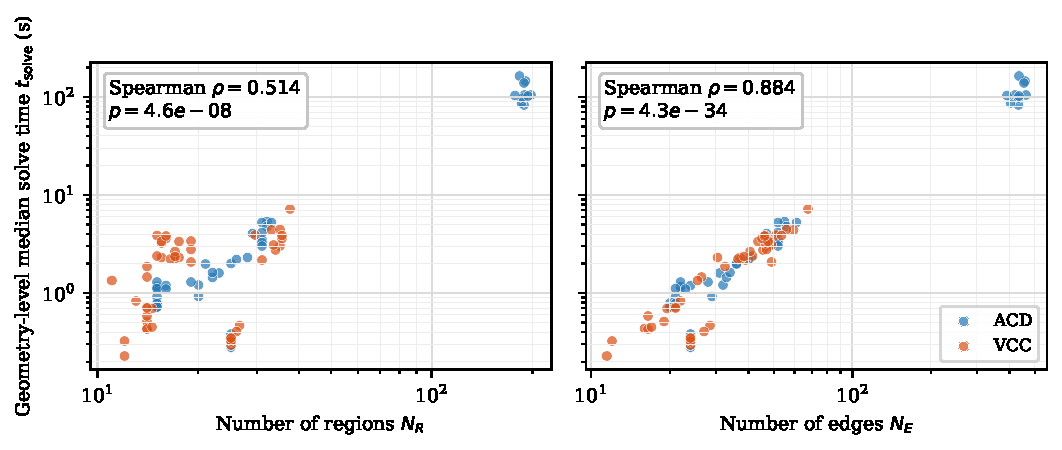
\includegraphics[width=\textwidth]{5-Experimental-results/figures/correlation_geometry_level.pdf}
\caption{Geometry-level relationships between graph size and solve time in the current benchmark ($n=100$ method--geometry observations). VCC contributes its within-geometry median over ten trials. Both axes are logarithmic; colors distinguish the decomposition methods. Reported coefficients and $p$-values are from two-sided Spearman rank-correlation tests.}
\label{fig:exp-correlations}
\end{figure}

This disparity follows from how a GCS program is assembled. A region contributes
a local copy of the continuous state and its within-set constraints, but each
directed edge introduces a flow variable together with edge-conditioned copies
of endpoint variables. For a B\'ezier trajectory, these copies are
high-dimensional because they carry control points and timing variables, and
their activation requires perspective formulations of continuity, derivative,
and cost constraints. Increasing $N_E$ therefore expands several coupled blocks
of variables and conic constraints per adjacency, not merely a scalar incidence
matrix. A dense graph also gives presolve more candidate flows and bounds to
propagate, weakens simple topological pruning when many alternate routes remain,
and enlarges the relaxation subsequently passed to rounding. The stronger
edge-count association is consequently consistent with $N_E$ acting as a
pre-construction proxy for this edge-bound algebraic workload, whereas $N_R$
does not encode how densely the regions intersect. Correlation alone does not
establish a causal scaling law, and the observations are pooled across map
families and methods; nevertheless, the formulation explains why
decompositions with similar $N_R$ can have markedly different solve times.

\subsection{Trajectory Quality}
Table~\ref{tab:exp-quality} reports trajectory medians and IQRs using the same
geometry-level aggregation. Path length does not identify a uniform winner:
the across-geometry paired median difference (ACD minus VCC) is $-0.144$, and a
two-sided Wilcoxon test provides no evidence of a method effect
($p_{\rm adj}=0.357$). The family-level differences are small on
\code{flappy} and \code{narrows}, favor VCC on \code{rooms}, and favor ACD on
\code{clustered} and \code{u\_shaped}.

\begin{table}[htbp]
\caption{Trajectory-quality metrics reported as median [Q1, Q3] across ten geometries. Failed trials are excluded from trajectory-dependent summaries.}
\label{tab:exp-quality}
\centering
\scriptsize
\setlength{\tabcolsep}{2.5pt}
\resizebox{\textwidth}{!}{%
\begin{tabular}{@{}llrrrr@{}}
\toprule
Map & Method & Path length & Traj. time & Min. clearance & Active regions \\
\midrule
Clustered & ACD & 7.62 [7.41,7.98] & 9.90 [9.78,10.48] & $7.43{\times}10^{-5}$ [$4.33{\times}10^{-5}$,$1.60{\times}10^{-4}$] & 16 [15,17.8] \\
          & VCC & 8.52 [8.46,8.60] & 8.91 [8.62,9.14] & $8.44{\times}10^{-2}$ [$5.92{\times}10^{-2}$,$1.54{\times}10^{-1}$] & 5.5 [4.3,6.8] \\
Narrows   & ACD & 16.35 [15.86,17.32] & 24.05 [23.90,24.43] & $3.66{\times}10^{-4}$ [$1.19{\times}10^{-4}$,$4.89{\times}10^{-4}$] & 13 [11.5,13.8] \\
          & VCC & 16.14 [15.76,16.35] & 25.87 [24.32,26.80] & $1.08{\times}10^{-3}$ [$7.05{\times}10^{-4}$,$1.65{\times}10^{-3}$] & 9 [9,9] \\
Rooms     & ACD & 7.55 [7.48,7.59] & 8.53 [8.19,8.68] & $1.06{\times}10^{-3}$ [$2.88{\times}10^{-4}$,$4.80{\times}10^{-3}$] & 11 [11,11.8] \\
          & VCC & 7.16 [7.16,7.26] & 7.03 [7.02,7.06] & $4.51{\times}10^{-3}$ [$3.41{\times}10^{-3}$,$5.31{\times}10^{-3}$] & 7 [7,7.5] \\
U-shaped  & ACD & 7.61 [7.55,8.00] & 7.96 [7.57,8.30] & $6.89{\times}10^{-4}$ [$3.03{\times}10^{-4}$,$1.58{\times}10^{-3}$] & 8 [7,9] \\
          & VCC & 8.10 [7.85,8.30] & 8.22 [8.06,8.38] & $2.11{\times}10^{-2}$ [$1.13{\times}10^{-2}$,$3.57{\times}10^{-2}$] & 5 [5,5.5] \\
Flappy    & ACD & 52.65 [52.56,52.76] & 71.32 [70.91,71.91] & $2.09{\times}10^{-4}$ [$7.98{\times}10^{-5}$,$4.45{\times}10^{-4}$] & 23 [23,23] \\
          & VCC & 52.81 [52.79,52.97] & 71.15 [70.76,71.50] & $2.49{\times}10^{-4}$ [$1.34{\times}10^{-4}$,$5.37{\times}10^{-4}$] & 25 [25,25] \\
\bottomrule
\end{tabular}
}
\end{table}

VCC has higher median minimum clearance in every family. The paired comparison
is significant after Holm correction ($p_{\rm adj}<9.3\times10^{-6}$), but the
effect is heterogeneous: VCC's clearance IQR is
$[5.92\times10^{-2},1.54\times10^{-1}]$ on \code{clustered} and
$[1.13\times10^{-2},3.57\times10^{-2}]$ on \code{u\_shaped}, compared with
$[1.34\times10^{-4},5.37\times10^{-4}]$ on \code{flappy}. The visibility cover
can therefore bias the optimizer toward routes supported by larger overlapping
free-space sets, but it does not impose a clearance objective and should not be
interpreted as a safety guarantee. Moreover, the clearance gain coexists with
higher decomposition time and reduced stochastic reliability in constrained
families. This is a Pareto trade-off rather than evidence that either
decomposition dominates in trajectory quality.

Relaxation behavior provides a second distinction. The corridor-like graphs in
the \code{flappy} family admit few meaningful route alternatives, so their relaxed
and rounded objectives remain close. In more highly connected
\code{clustered} graphs, fractional flow can distribute over competing routes,
increasing the relaxation--rounding gap even after VCC reduces graph size.
Hence, graph compactness, relaxation tightness, and geometric clearance are
related but non-equivalent properties of a decomposition.

\subsection{Visual Evidence on Flappy Maps}
The \code{flappy} family provides a qualitative stress test because every route
must alternate between upper and lower openings. Figure~\ref{fig:exp-flappy}
shows four representative geometries. Both decompositions preserve the
mandatory corridor sequence, consistent with their nearly equal median path
lengths (52.65 for ACD and 52.81 for VCC) and traversal times (71.32~s and
71.15~s). The images therefore corroborate geometric feasibility and route
similarity, but they do not establish statistical equivalence.

\begin{figure}[htbp]
\centering
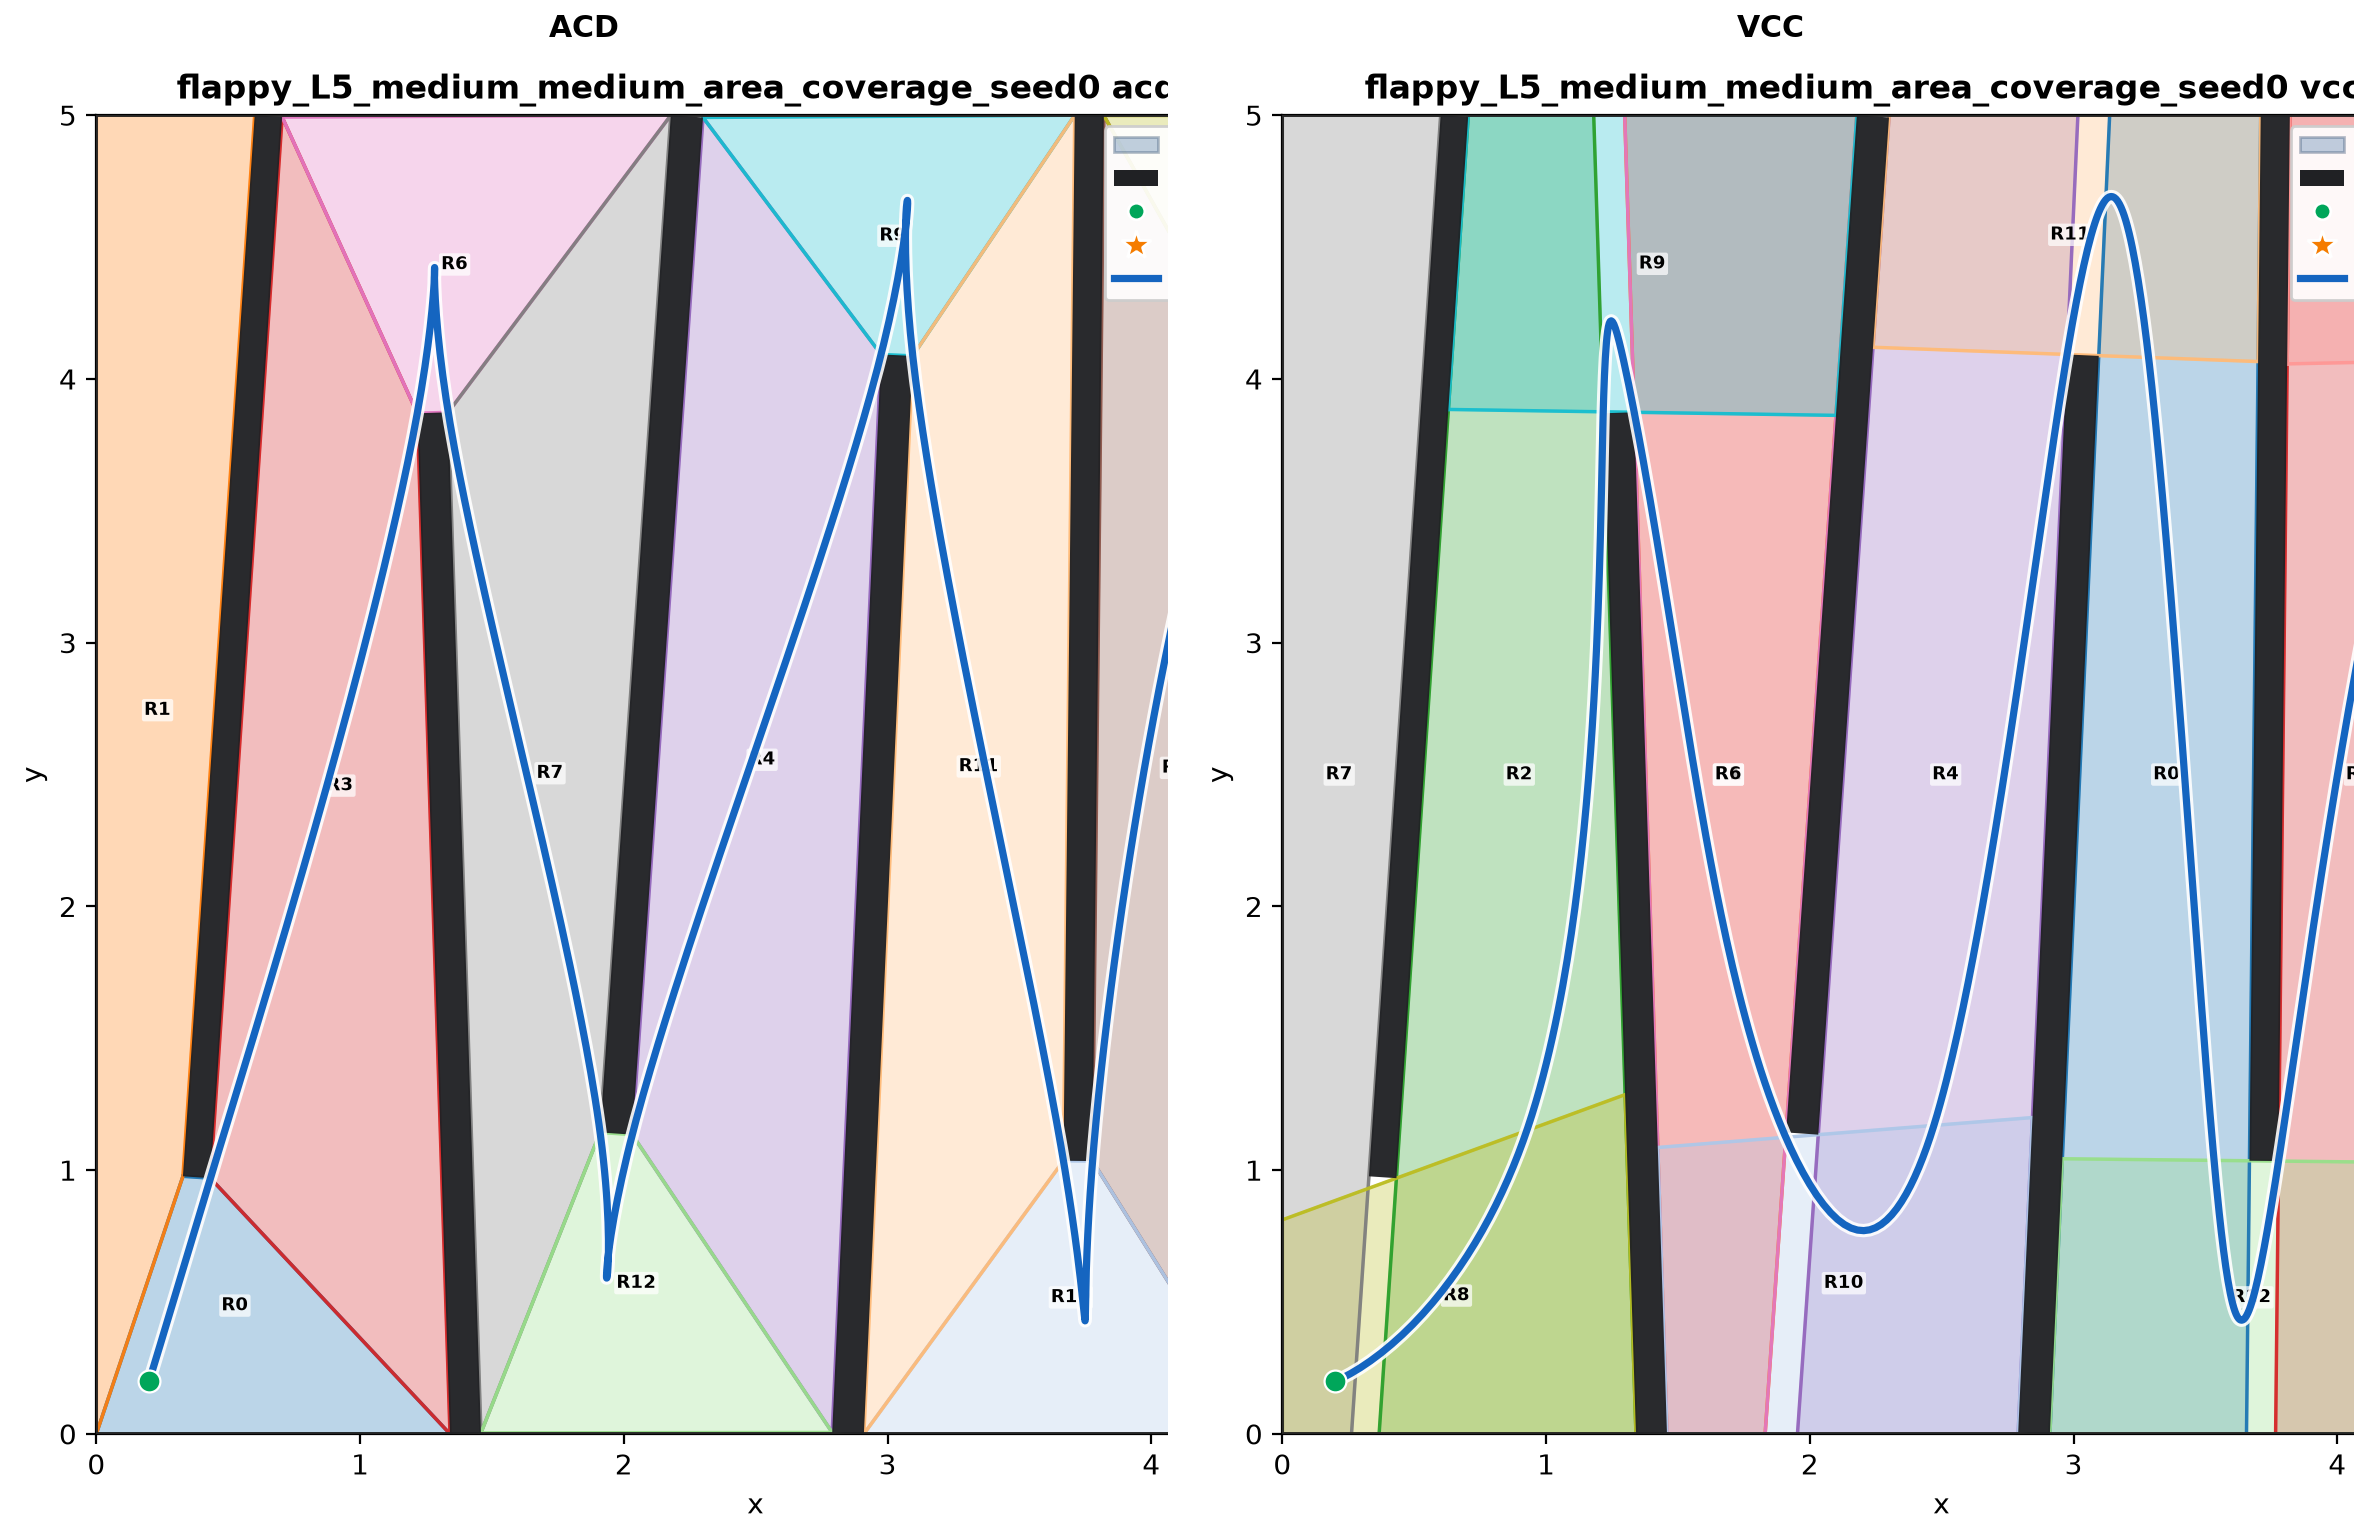
\includegraphics[width=0.48\textwidth]{5-Experimental-results/figures/flappy_seed0_comparison.png}
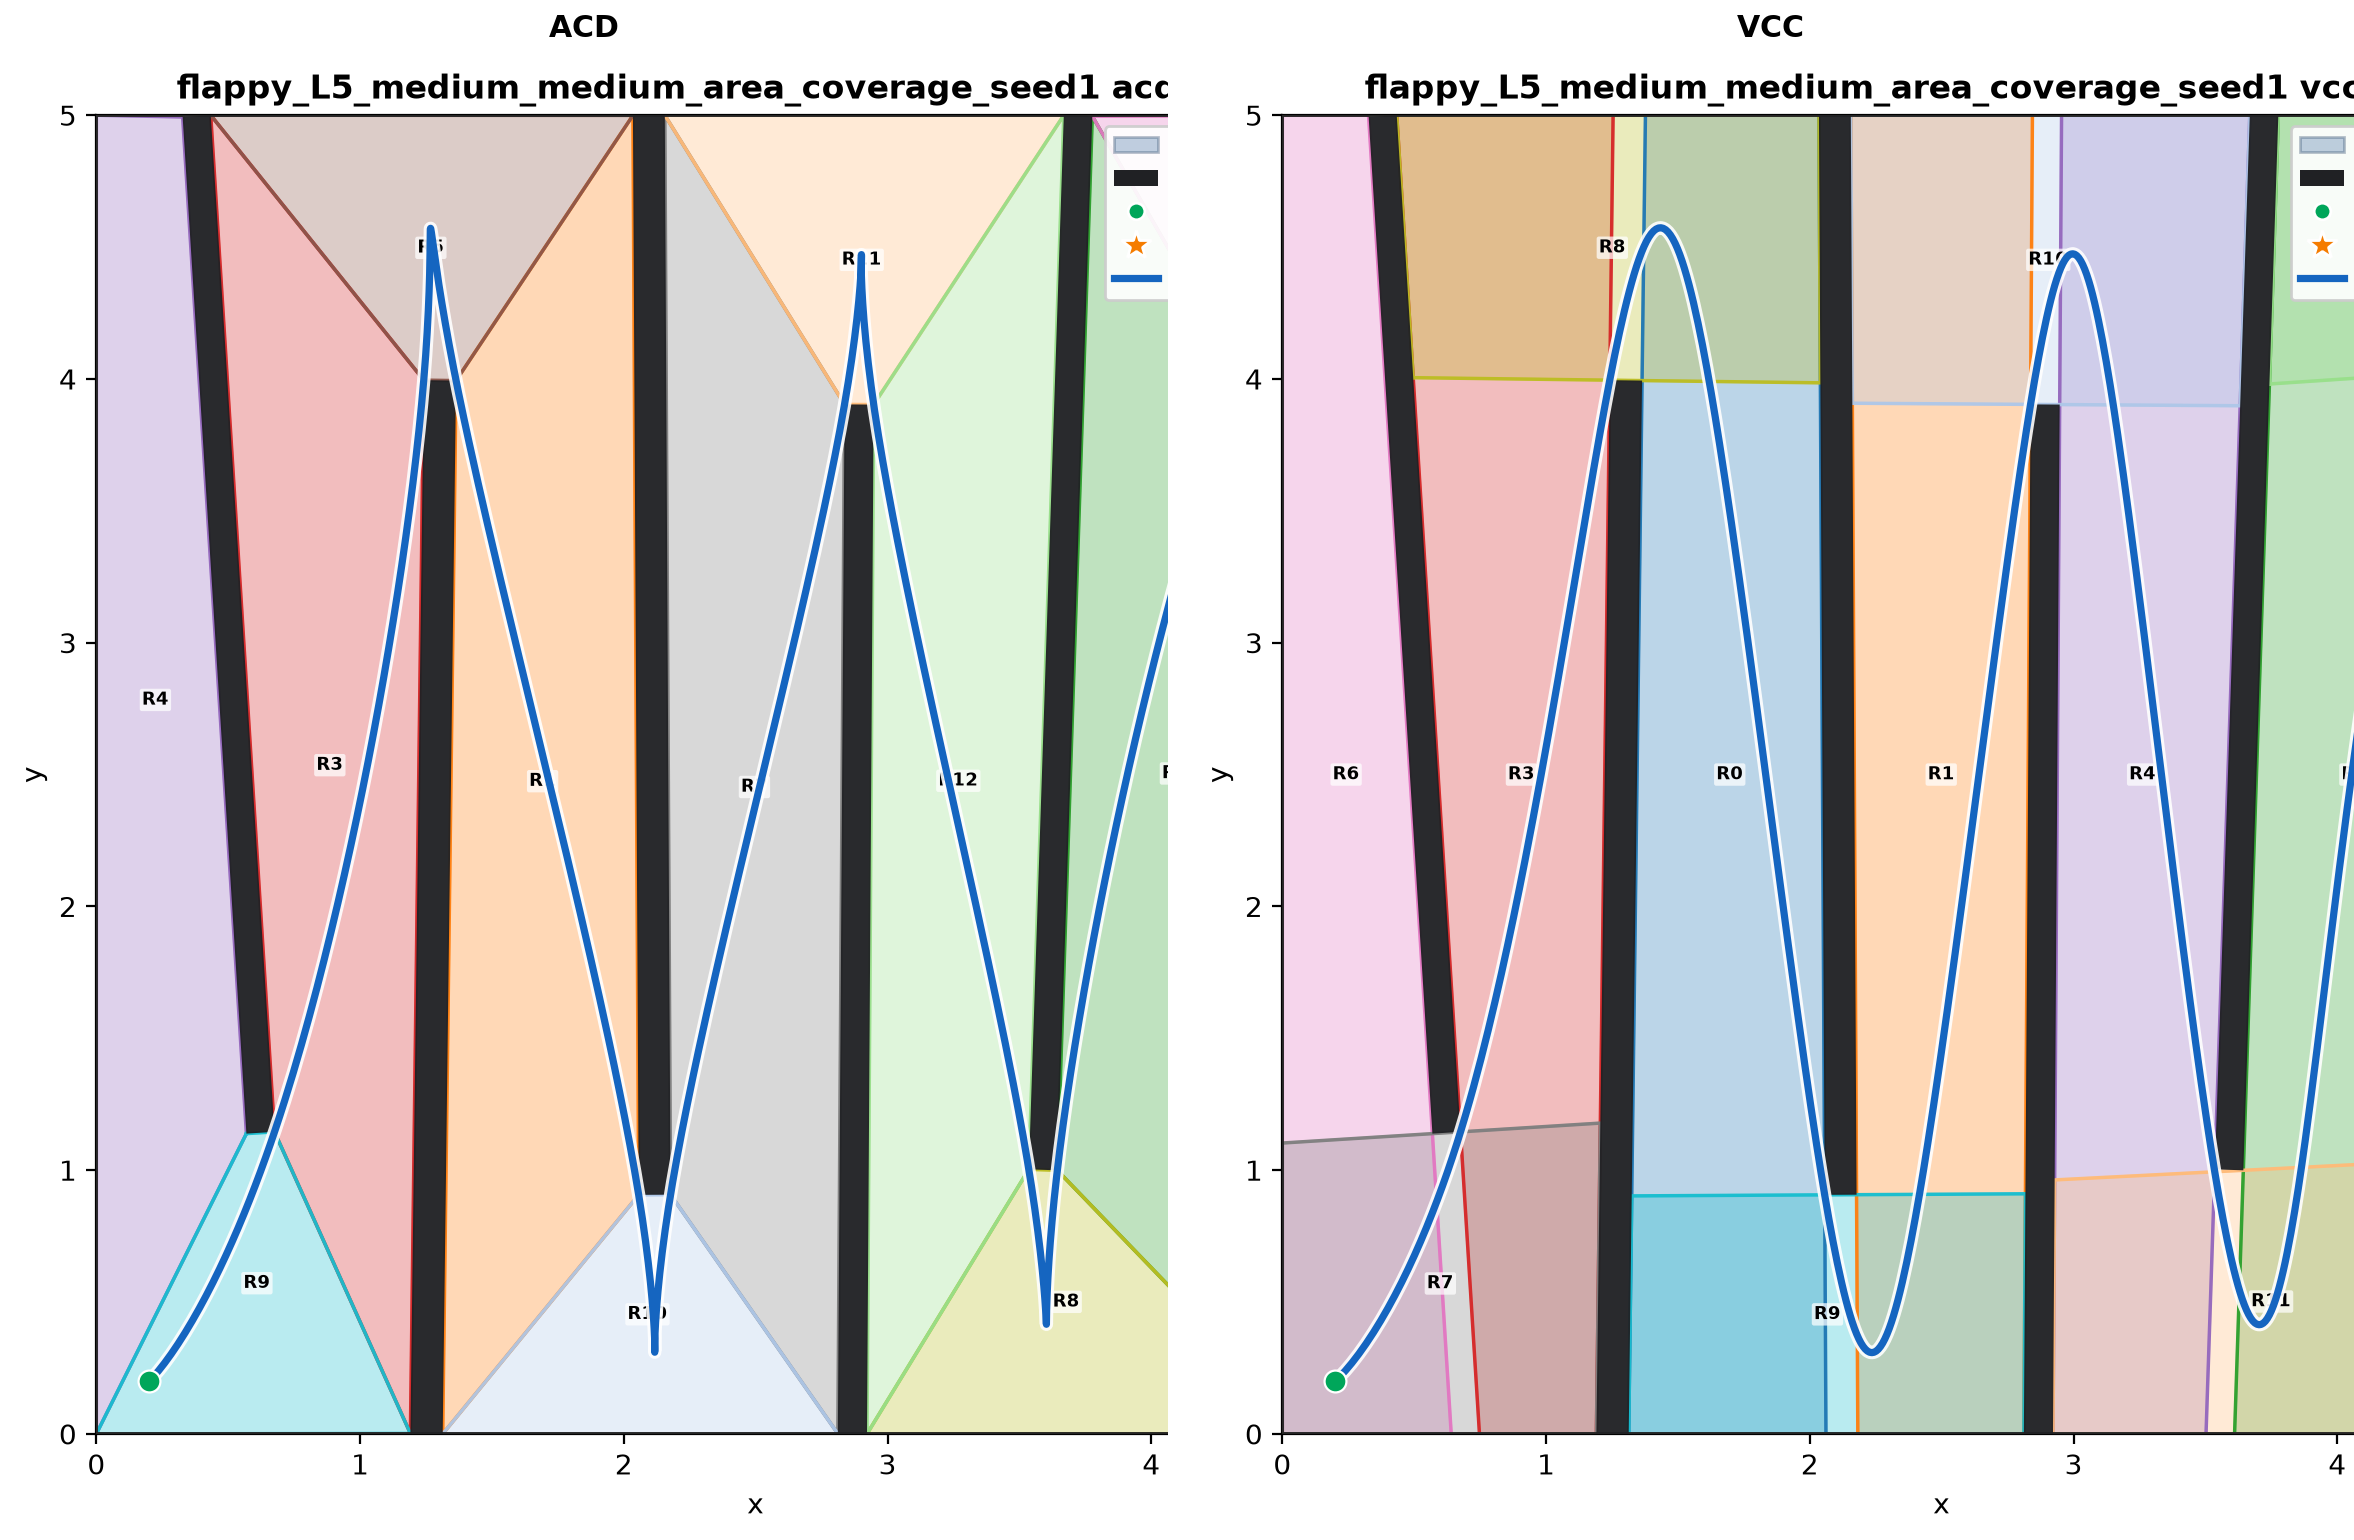
\includegraphics[width=0.48\textwidth]{5-Experimental-results/figures/flappy_seed1_comparison.png}
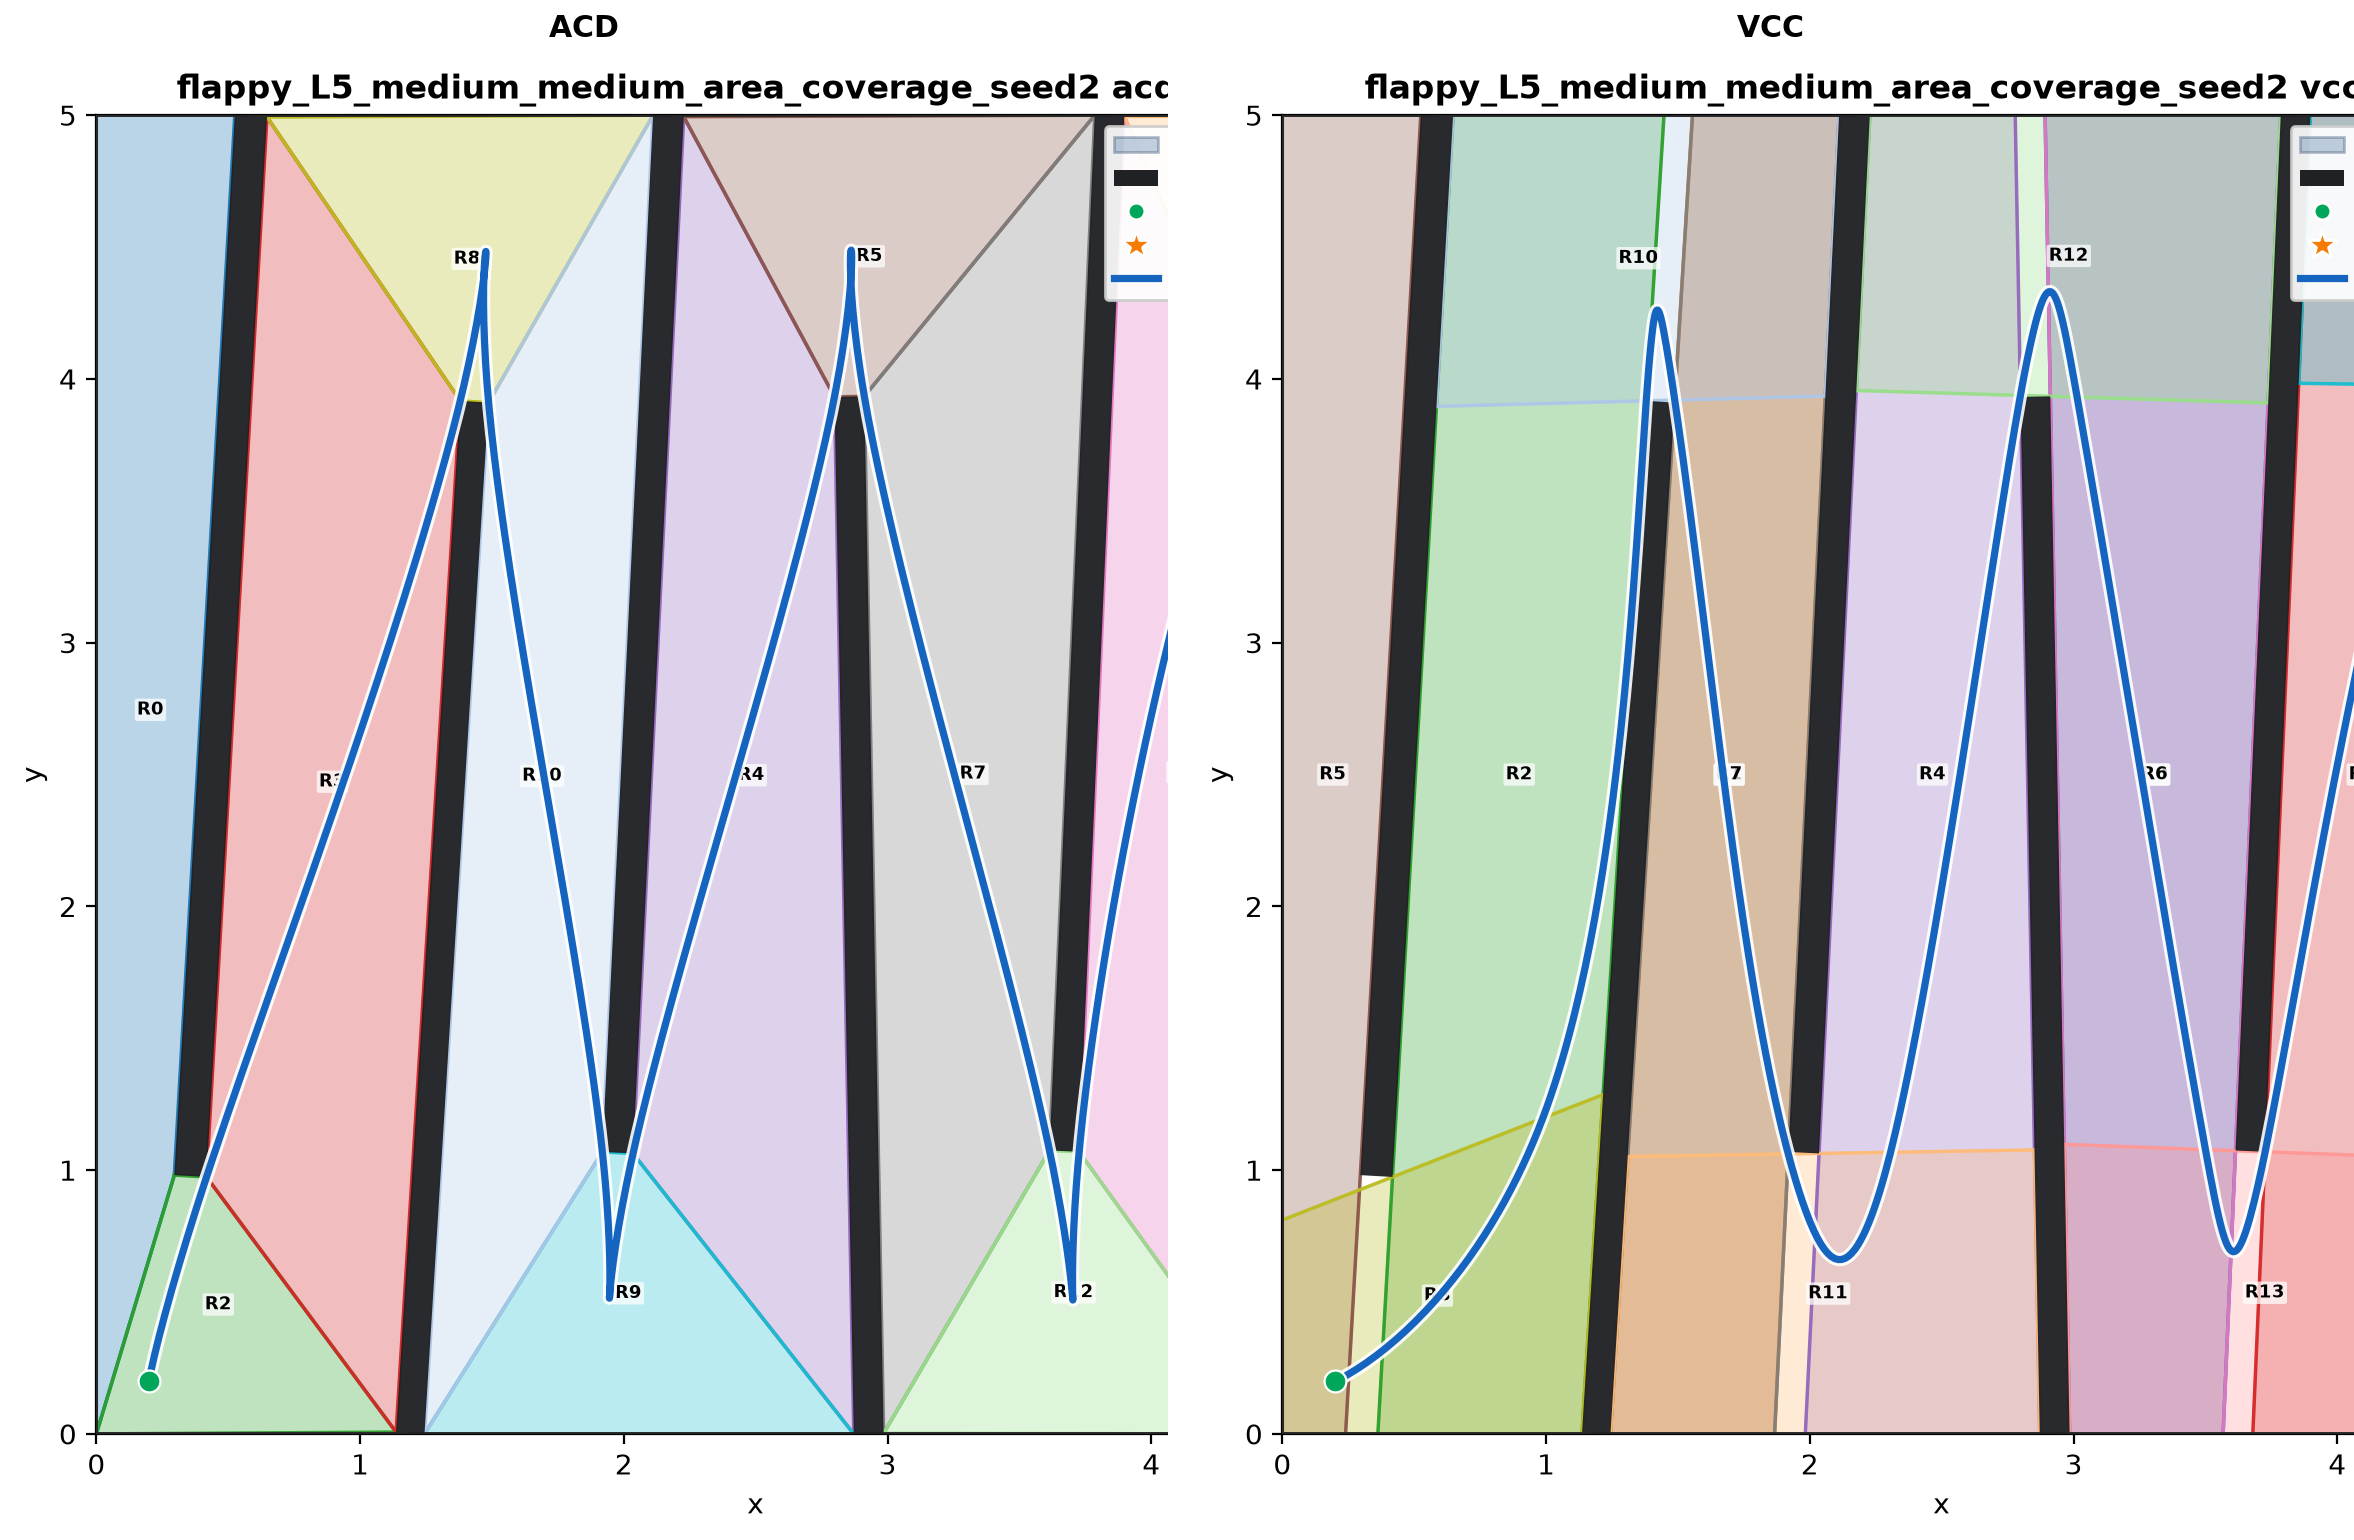
\includegraphics[width=0.48\textwidth]{5-Experimental-results/figures/flappy_seed2_comparison.png}
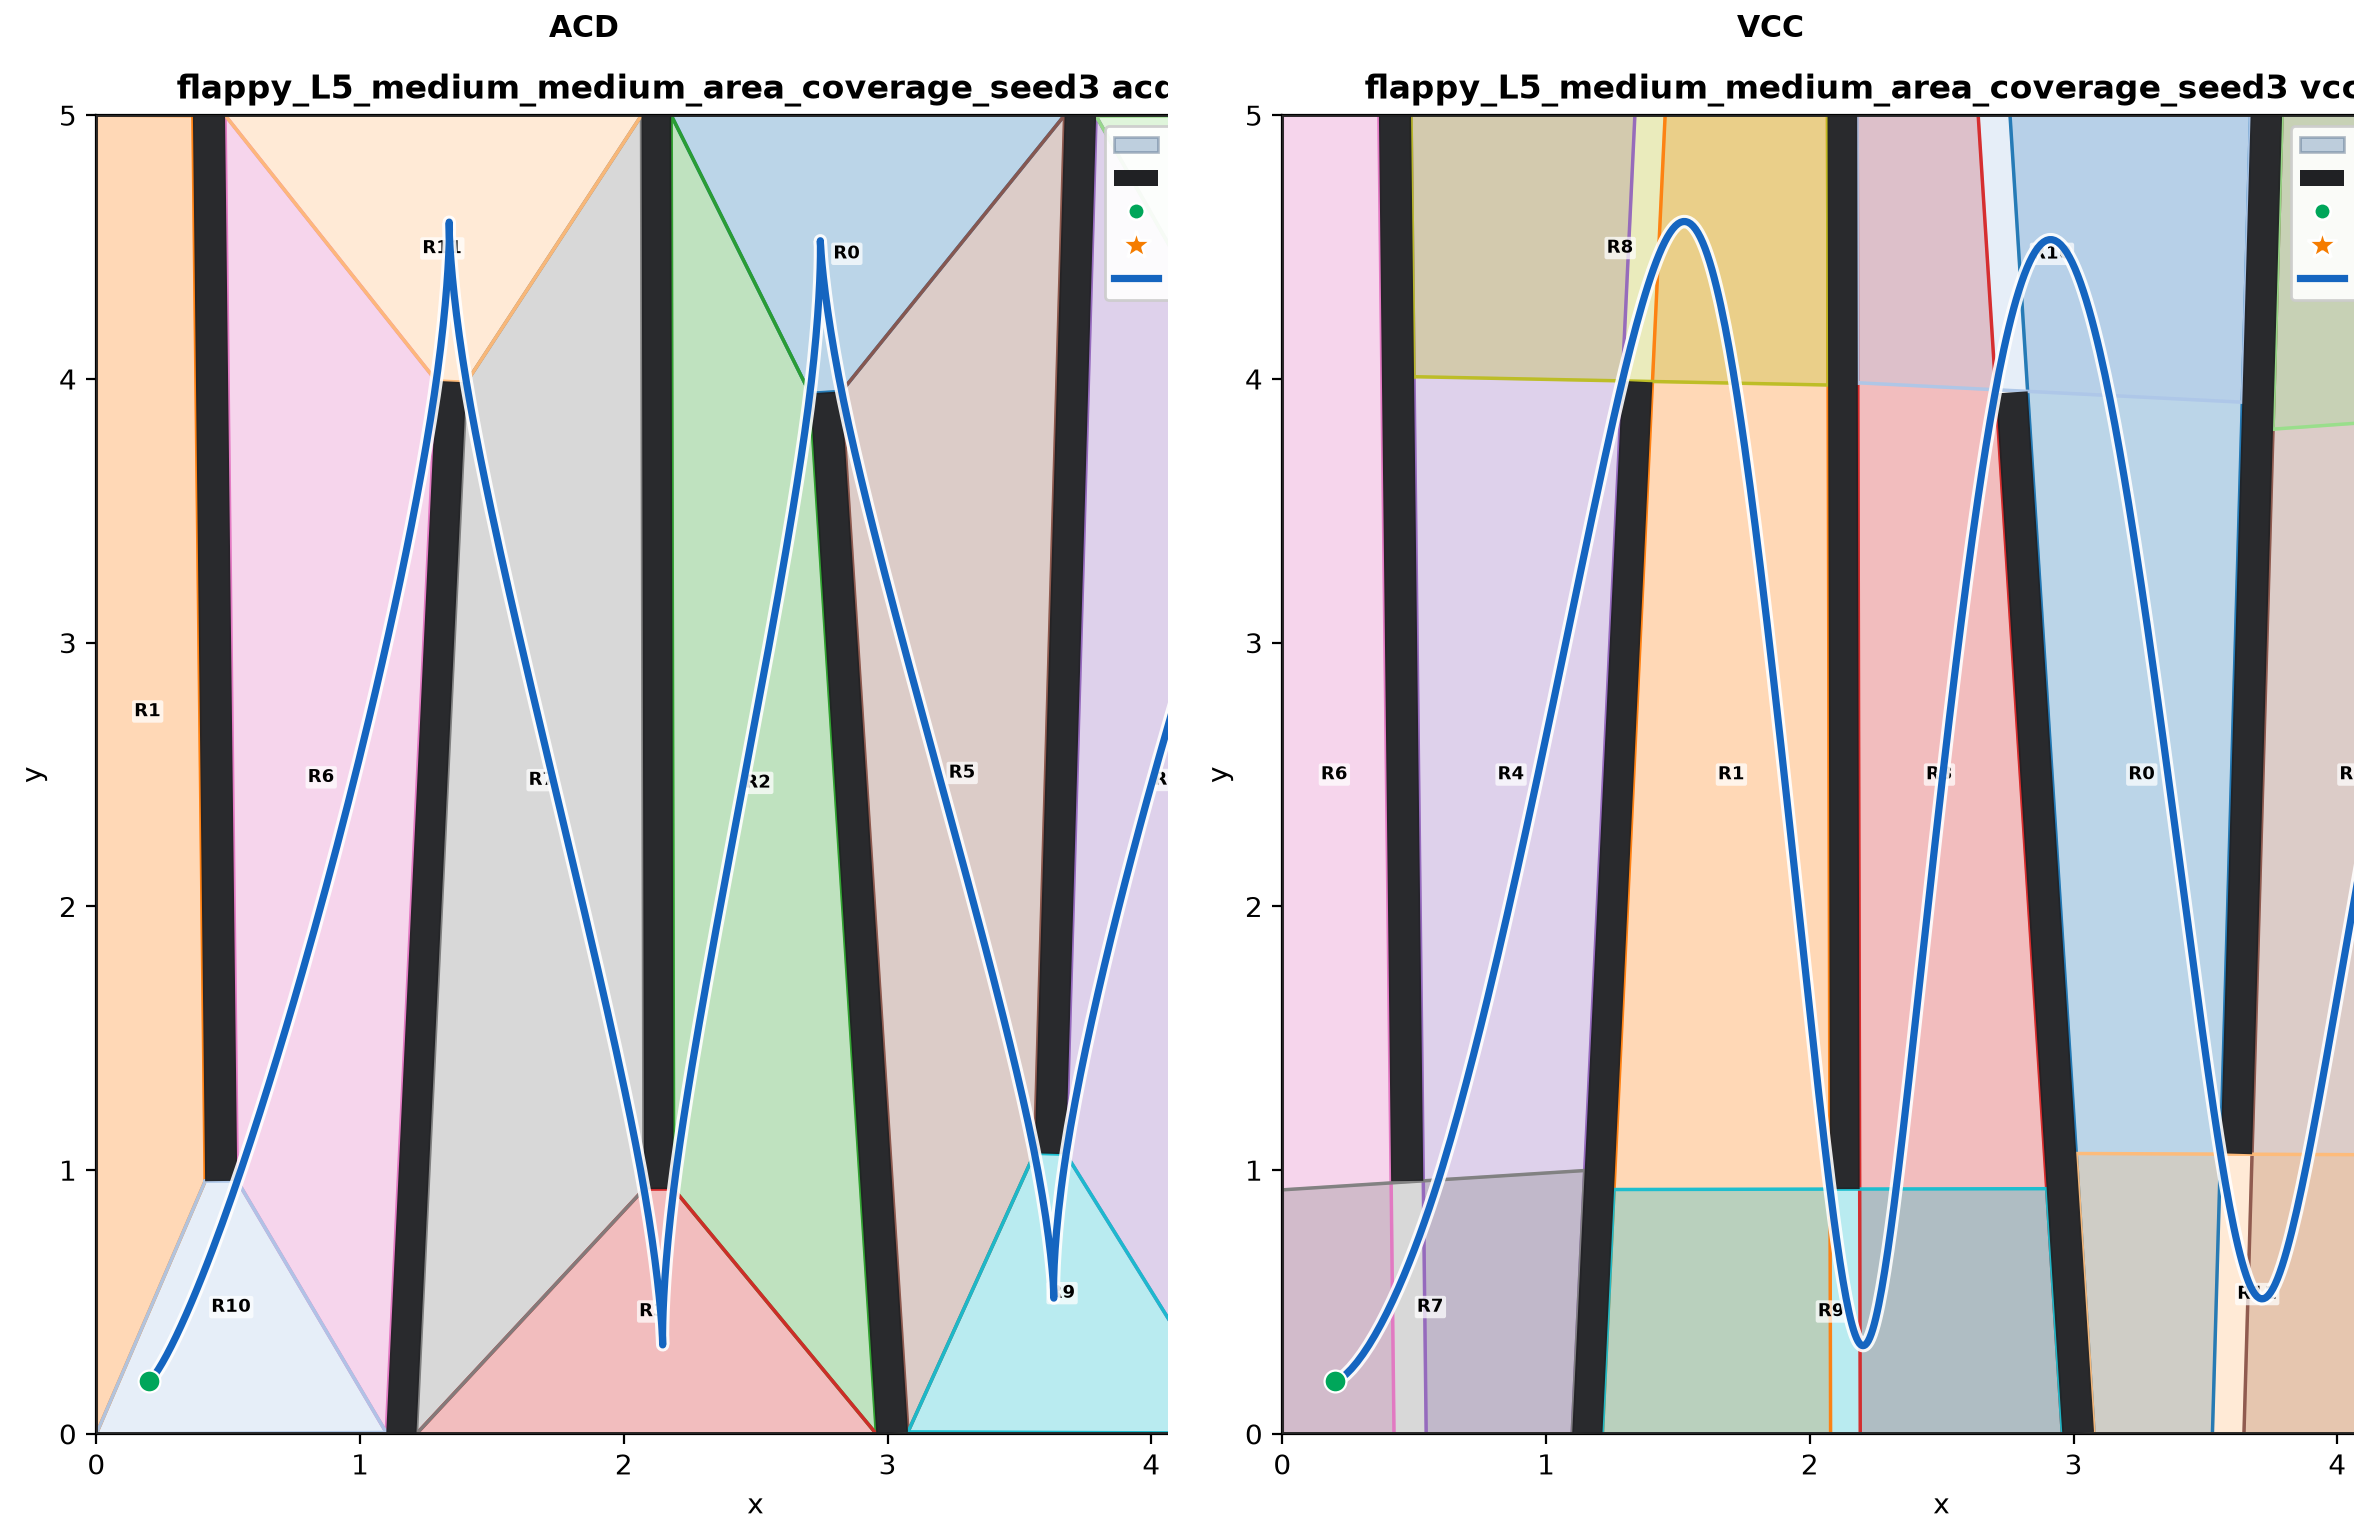
\includegraphics[width=0.48\textwidth]{5-Experimental-results/figures/flappy_seed3_comparison.png}
% 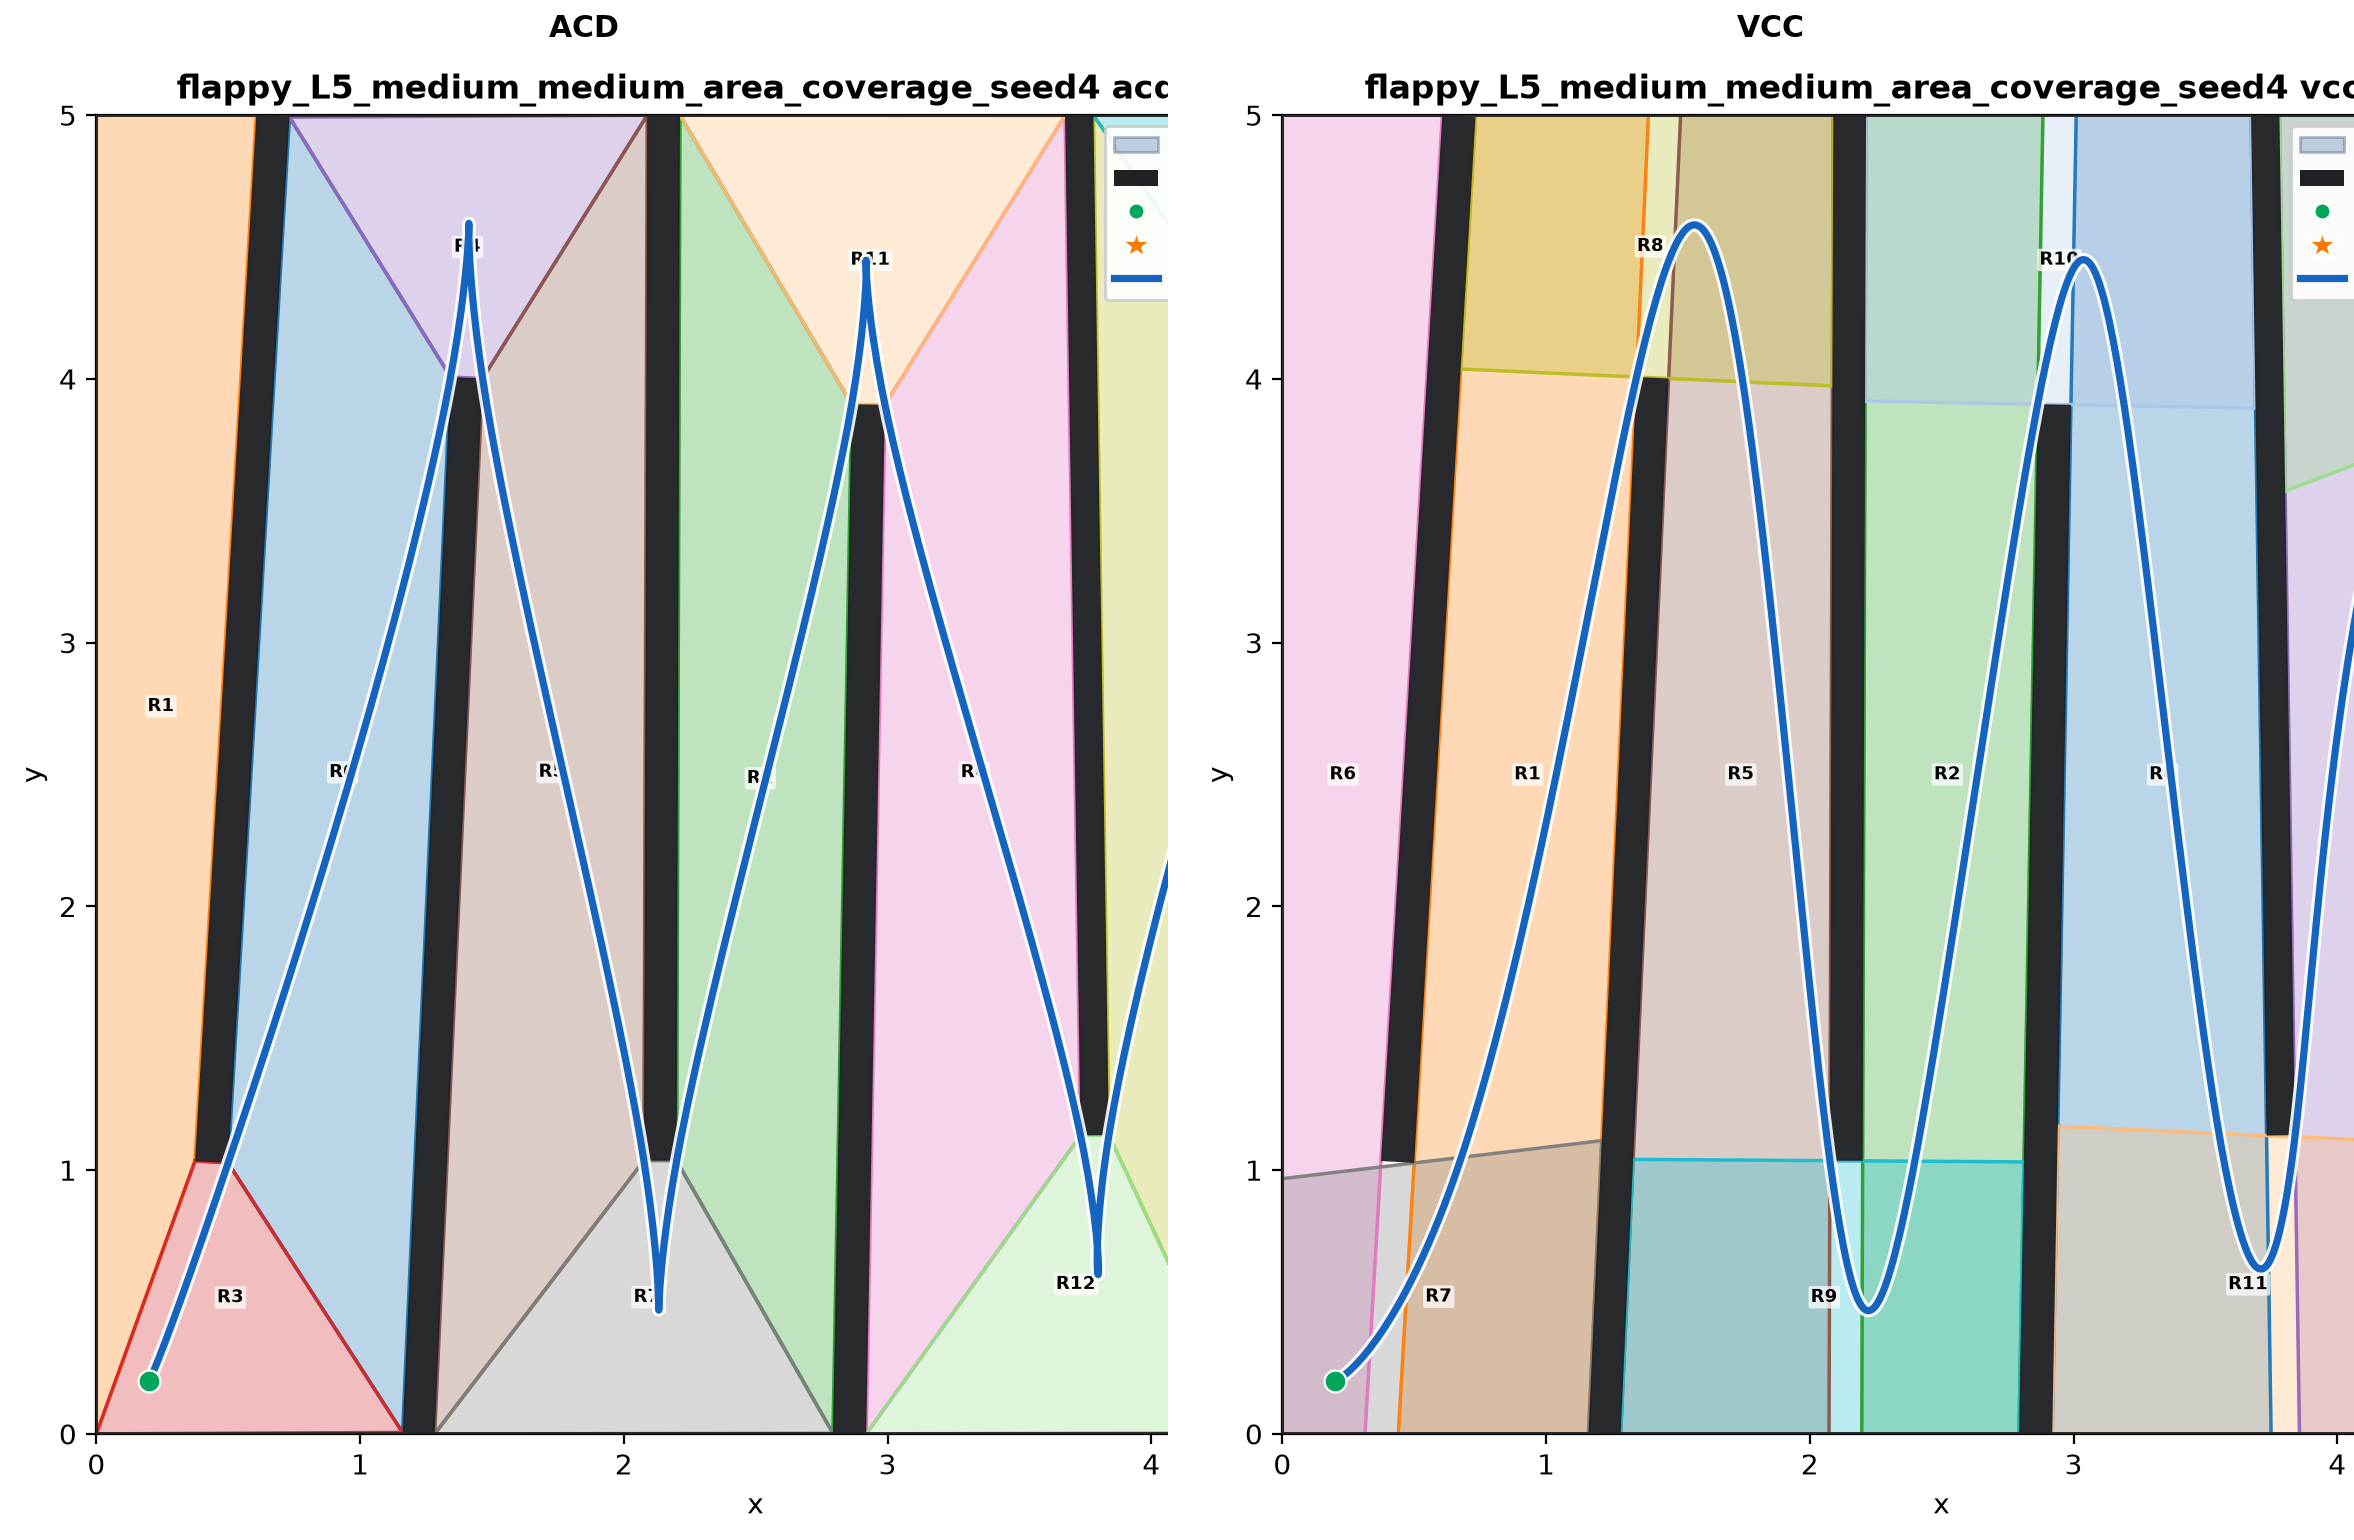
\includegraphics[width=0.48\textwidth]{5-Experimental-results/figures/flappy_seed4_comparison.png}
\caption{ACD and VCC comparisons on four representative \code{flappy} geometries. Obstacles are black, convex regions are colored, and the GCS trajectory is plotted in blue.}
\label{fig:exp-flappy}
\end{figure}

The principal difference is computational rather than geometric. ACD's median
end-to-end time is 2.08~s (IQR $[2.07,2.13]$~s), whereas VCC requires 21.87~s
(IQR $[21.75,22.19]$~s), almost entirely because of decomposition. Since both
methods induce the same median graph size ($N_R=25$, $N_E=24$), this family is
a controlled example in which VCC pays its sampling and clique-cover overhead
without obtaining a smaller online optimization problem.

\subsection{Discussion and Limitations}
The experiments identify the induced edge structure, rather than the number of
convex regions alone, as the most informative decomposition-level predictor of
GCS cost. VCC is advantageous online when visibility-based aggregation removes
both regions and adjacencies, as on \code{clustered} and \code{rooms}; it loses
that advantage when aggregation leaves a dense overlap graph, as on
\code{u\_shaped}, or leaves the graph essentially unchanged, as on
\code{flappy}. These results motivate reporting $N_E$, presolved program size,
relaxation and rounding behavior, and reliability alongside $N_R$.

The appropriate method consequently depends on query regime. For a single
start--goal query, ACD dominates end-to-end runtime in every tested family and
also achieves a 50/50 geometry success rate. VCC becomes attractive when the
environment decomposition is reusable: its one-time cost can be amortized over
multiple start--goal pairs, changes in trajectory boundary conditions, or
repeated replanning on a static map. If $t_{\rm dec}^{A}$ and
$t_{\rm dec}^{V}$ denote decomposition costs and $t_{\rm GCS}^{A}$ and
$t_{\rm GCS}^{V}$ denote per-query solve costs, VCC breaks even after
approximately
\(
Q^{\star}=(t_{\rm dec}^{V}-t_{\rm dec}^{A})/
(t_{\rm GCS}^{A}-t_{\rm GCS}^{V})
\)
queries whenever $t_{\rm GCS}^{A}>t_{\rm GCS}^{V}$. The family medians give
$Q^{\star}\approx2$ for \code{clustered} and $Q^{\star}\approx6$ for
\code{rooms}; no positive break-even point exists for families in which VCC
does not reduce per-query GCS time. This calculation assumes that the graph can
be reused without rebuilding and excludes any query-dependent preprocessing.

The clearance results expose a separate design trade-off. VCC often returns
trajectories with greater sampled minimum clearance, plausibly because larger
visibility cliques provide broader overlapping sets through which the
continuous trajectory can move. Achieving those sets requires extensive
visibility sampling and clique construction, however, and global coverage does
not ensure that every narrow gateway is represented robustly. A decomposition
selected for clearance may therefore incur both additional offline cost and
stochastic connectivity risk. Applications should treat coverage, graph
connectivity, and clearance as distinct acceptance criteria.

Several limitations bound these conclusions. First, the 50 geometries cover one
workspace scale, density level, obstacle-size level, VCC sample budget (500),
and coverage target (0.96). Second, the supplied summary CSVs retain quartiles
and population variance but omit trial-level certificate fields and failure
messages; consequently, the proposed narrow-gateway mechanism cannot be
verified without the raw logs. Third, the reported Wilcoxon tests operate on
geometry-level VCC medians to avoid pseudoreplication, but larger geometry sets
and paired bootstrap confidence intervals are needed for precise effect
estimation within each family. Finally, sampled minimum clearance is sensitive
to trajectory discretization and is not a continuous-time collision
certificate. Future experiments should vary sampling budget, target coverage,
workspace scale, and obstacle density; retain stage-resolved failures; evaluate
graph connectivity before optimization; and measure amortized performance over
explicit multi-query workloads.


%
%
\section{Conclusion and Future Work}
\label{sec:conclusion}

This paper compared ACD and VCC as alternative convex-cover front ends for the
same GCS--B\'ezier motion-planning pipeline. We have shown that, across 25 paired
instances, ACD solved every instance and VCC solved 23, with both failures in the
\code{narrows} family. VCC substantially reduced the downstream graph on the
\code{clustered} maps, but its decomposition cost made it slower end-to-end in
all five map families under the tested single-query configuration. Across the
48 successful runs, edge count was more strongly correlated with GCS solve time
than region count, highlighting the importance of evaluating the connectivity
induced by a convex cover rather than its number of regions alone.

These findings are limited to planar environments, five seeds per map family,
and one fixed set of decomposition and sampling parameters. Future work should
vary workspace scale, obstacle density, VCC sampling budget, and coverage target;
report uncertainty across a larger collection of instances; and evaluate
settings in which a decomposition is reused across multiple planning queries.
Such experiments would clarify when VCC's smaller downstream model offsets its
higher construction cost and whether the observed clearance differences persist
under broader conditions.

\begin{credits}
\subsubsection{\ackname} We acknowledge Ho Chi Minh City University of Technology (HCMUT), VNU-HCM for supporting this study.
\end{credits}
\bibliographystyle{splncs04}
\bibliography{mybibliography}
\end{document}
